\documentclass{article}
\usepackage{graphicx}
\usepackage[dvipsnames,table]{xcolor}
\usepackage[utf8]{inputenc}
\usepackage{siunitx}
\usepackage[american,siunitx]{circuitikz}
\usepackage{amsmath}
\usepackage{svg}
\usepackage{booktabs}
\usepackage{float}
\usepackage{xparse, xfp}
\usepackage{multirow}
\usepackage{tikz}
\usepackage{karnaugh-map}
\usepackage{pdfpages}
\usepackage{hyperref}
\hypersetup{
    colorlinks=true,
    linkcolor=blue,
    filecolor=magenta,      
    urlcolor=cyan,
}
\usetikzlibrary{calc}
%\usepackage[landscape]{geometry}
\renewcommand{\thesubsection}{\thesection.\alph{subsection}}
\newcommand{\equal}{=}
\newcommand{\greyrule}{\arrayrulecolor{black!30}\midrule\arrayrulecolor{black}}
\makeatletter
\newcommand\currcoor{\the\tikz@lastxsaved,\the\tikz@lastysaved}
\makeatother
\newcolumntype{:}{@{\hskip\tabcolsep\color{black!30}\vrule\hskip\tabcolsep}}

\ExplSyntaxOn
\NewExpandableDocumentCommand \groupify { O{\,\allowbreak} m m }
  { \jakob_groupify:nnn {#1} {#2} {#3} }
\cs_new:Npn \jakob_groupify:nnn #1 #2 #3
  { \__jakob_groupify_loop:nnw { 1 } {#2} #3 \q_recursion_tail {#1} \q_recursion_stop }
\cs_new:Npn \__jakob_groupify_loop:nnw #1 #2 #3
  {
    \quark_if_recursion_tail_stop:n {#3}
    \exp_not:n {#3}
    \int_compare:nNnTF {#1} = {#2}
      { \__jakob_groupify_sep:n }
      { \exp_args:Nf \__jakob_groupify_loop:nnw { \int_eval:n { #1+1 } } }
          {#2}
  }
\cs_new:Npn \__jakob_groupify_sep:n #1 #2 \q_recursion_tail #3
  {
    \tl_if_empty:nF {#2} { \exp_not:n {#3} }
    \__jakob_groupify_loop:nnw { 1 } {#1}
    #2 \q_recursion_tail {#3}
  }
\ExplSyntaxOff

%\title{ECE 3301\\Introduction to Microcontrollers\\\,\\Assignment 2}
%\author{Choi Tim Antony Yung}
\begin{document}
%\maketitle

%\thispagestyle{empty}
%\setcounter{page}{0}

%\newpage

\section{(30) What is the difference between:}
\subsection{Program counter and memory address register? (10)}
Program counter stores the address of instruction whereas memory address register stores the address of data. More specifically, PC typically stores the address of the next instruction to be executed. 

\newpage
\subsection{Accumulator and Instruction Register? (10)}
Accumulator store data whereas Instruction Register store instruction. More specifically, Accumulator typically store one of the operand before and the result after arithmetics or logic operations; and the instruction register stores instruction to be executed after it was fetched by the CPU.

\newpage
\subsection{General Purpose Register (GPR) based CPU and an Accumulator (ACC) based CPU? (10)}
In accumulator-based microcontroller such as the PIC18F, all ALU operations are performed using the Accumulator as one of the data sources, whereas in general-purpose register based microcontroller such as the MSP430, any general-purpose register can be used as an accumulator.

\newpage

\section{(40) Use the PIC18F simulator to calculate the following operations:}
Calculate the difference and sum manual calcualtons. Program the problem using assembly code and submit a snap shot of the status register (digit carry, sign, carry, zero, and overflow flags) and the file register showing the result. Did they match?
\subsection{$A7_{16}-A7_{16}$ (20)}
As seen in the following screenshot, the result of manual calculation done in the comments matches the difference stored at 0x50 and the status flags in status register after the calculation is done.
\begin{figure}[H]
  \centering
  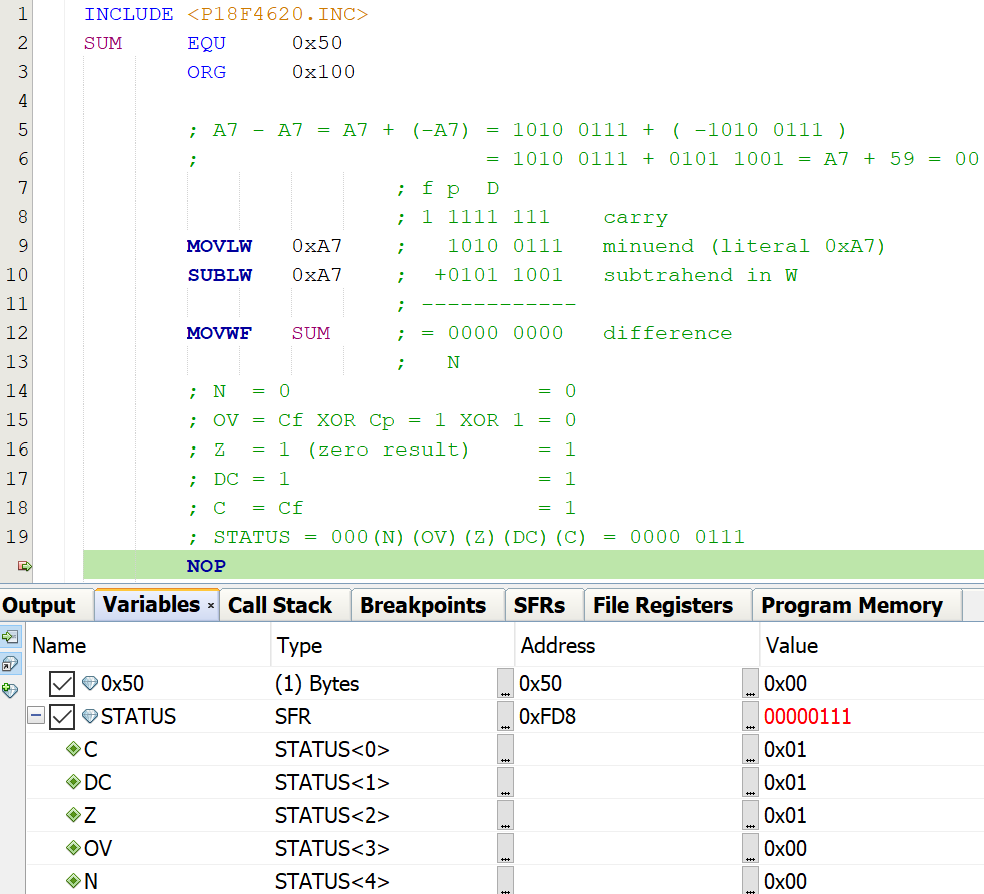
\includegraphics[width=\textwidth]{ECE3301_Assignment2_Sub.png}
  \caption{Manual calculation in comment, state of status register and at 0x50}
\end{figure}
\subsection{$6E_{16}+3A_{16}$ (20)}
As seen in the following screenshot, the result of manual calculation done in the comments matches the sum stored at 0x50 and the status flags in status register after the calculation is done.
\begin{figure}[H]
  \centering
  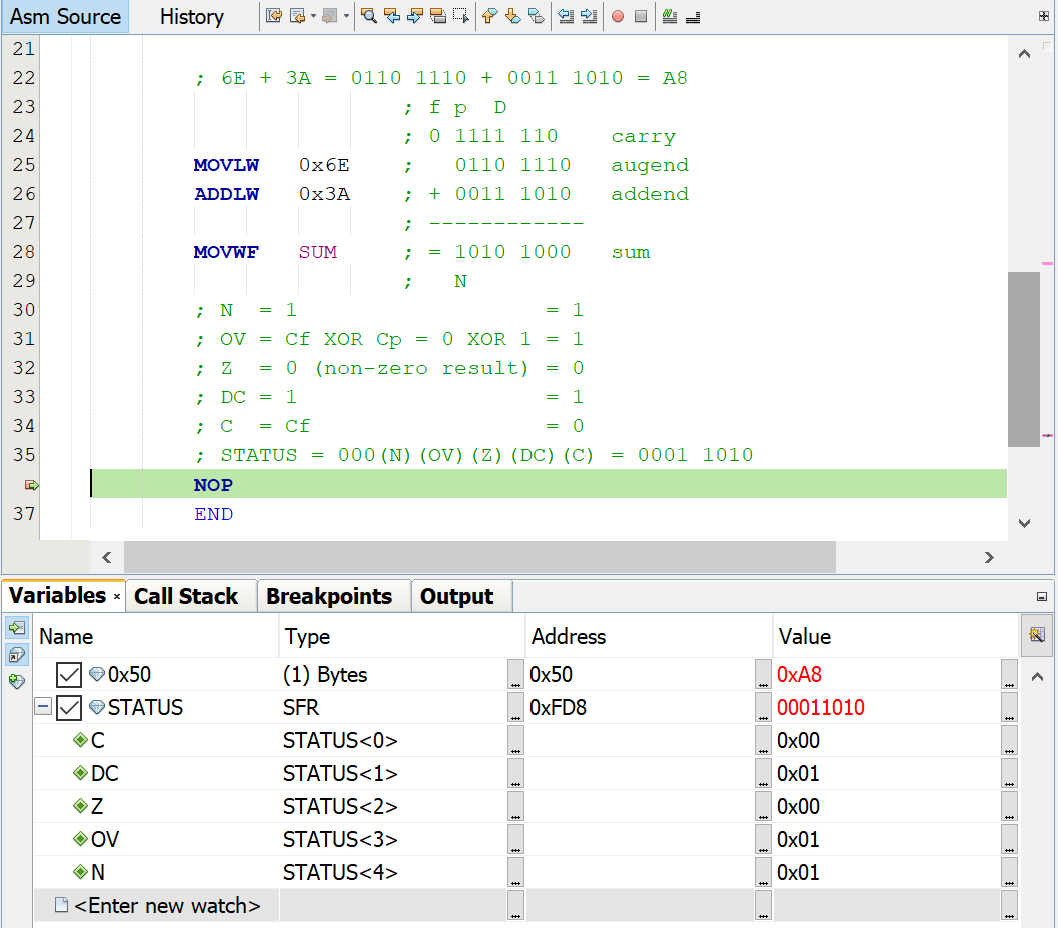
\includegraphics[width=\textwidth]{ECE3301_Assignment2_Add.png}
  \caption{Manual calculation in comment, state of status register and at 0x50}
\end{figure}

\newpage

\section{(30) What is the difference between PUSH and POP operations in the stack? How is the stack accessed and what effect the access have on addressing the stack memory locations?}


\subsection*{In microcontrollers where the stack is accessed from the top (lowest address):}
\begin{itemize}
\item Stack Pointer (STKPTR) register points to the address of data at the top (lowest address) of the stack.
\item PUSH write to the top of the stack whereas POP read from the top of the stack.
\item PUSH decrement the STKPTR to point to the next top (lowest address) and write data to that address.
\item POP read the item at the top (lowest address) that is being pointed by STKPTR and increment the STKPTR to point to the next data in the stack at the top (lowest address)
\end{itemize}

\subsection*{In microcontrollers where the stack is accessed from the bottom (highest address):}
\begin{itemize}
\item Stack Pointer (STKPTR) register points to the address of data at the bottom (highest address) of the stack.
\item PUSH write to the bottom of the stack whereas POP read from the bottom of the stack.
\item PUSH increment the STKPTR to point to the next bottom (highest address) and write data to that address.
\item POP read the item at the bottom (highest address) that is being pointed by STKPTR and decrement the STKPTR to point to the next data in the stack at the bottom (highest address)
\end{itemize}

\end{document}
